\chapter{System design and implementation}
\label{c:system-design-and-implementation}

\if 0
\bibliography{thesis}
\graphicspath{{./figsrc/}}
\fi

\section{System overview}
% 講大概的圖是在幹麼
Fig.~\ref{fig:big-system} shows the schematic diagram of the whole system. We will first introduce smart farm platform because this is where we implement our system. Second, we briefly introduce each components in the system. Third, we will describe the user cases which we designed and the sequence diagram behind each case, including critical case. At last, we focus on the detail design of PI and recording server.

\begin{figure}[H]
    \centering
    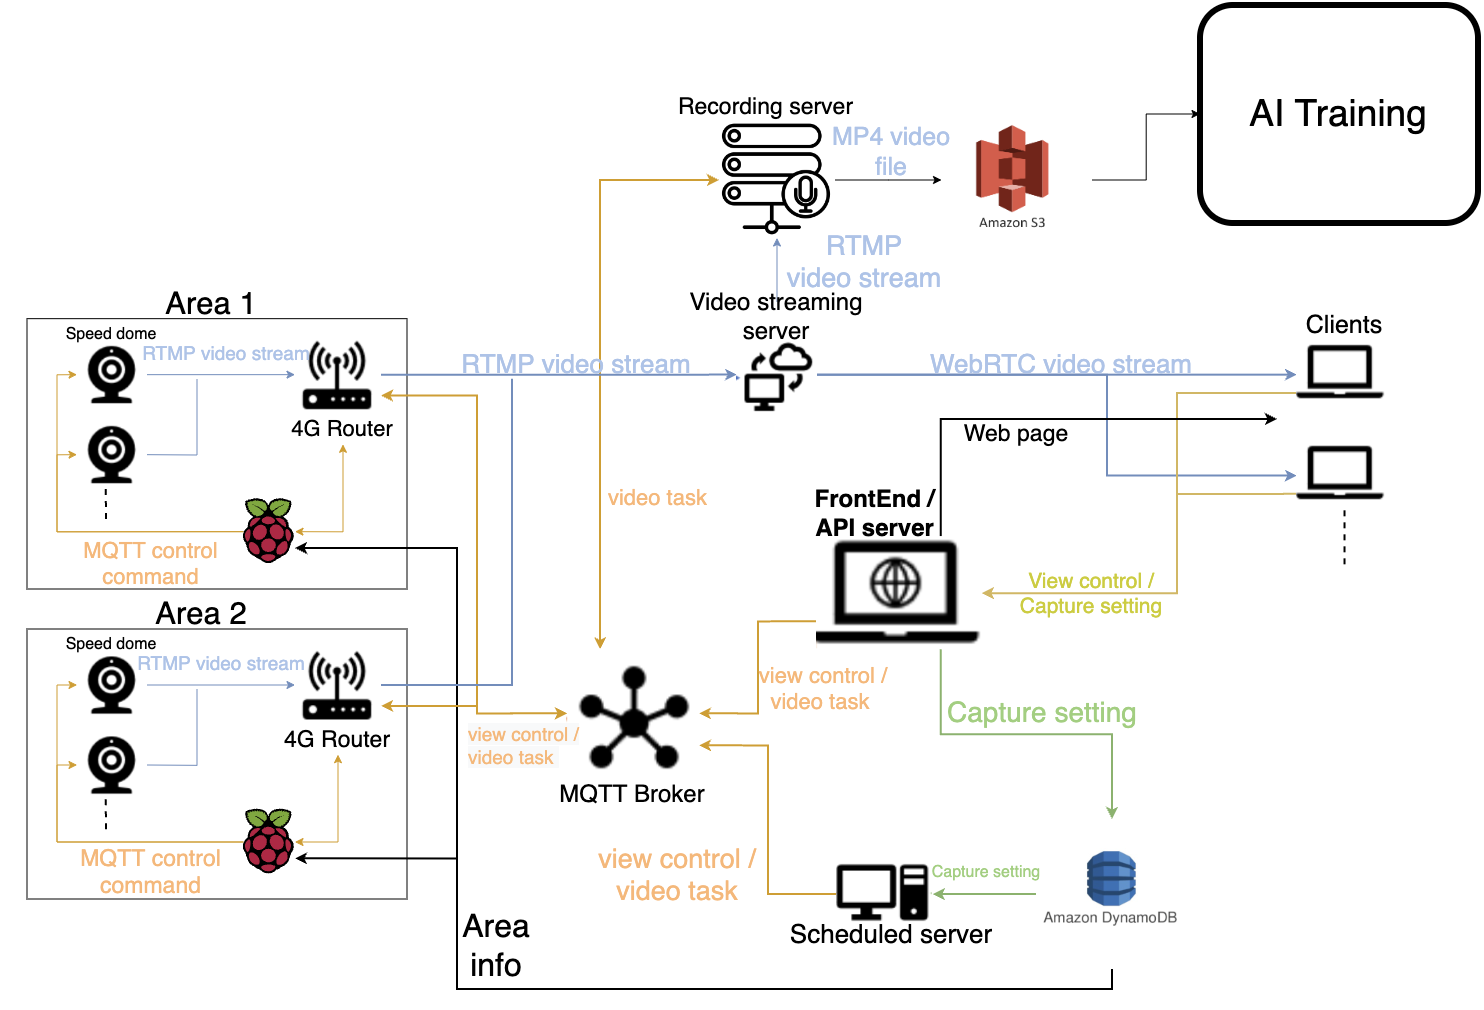
\includegraphics[width=\textwidth]{figsrc/big-system.png}
    \caption{Schematic diagram of system\label{fig:big-system}}
\end{figure}

\section{Smart farm platform}
Smart Farming Platform~\cite{agri-web} is established by National Tsing Hua University High Speed Network Lab(HSNL). HSNL installed sensor and camera on site in order to capture data such as image, live stream, soil moisture or any other sensor data. Process data and upload it to platform then show on webpage for expert to analyze or used as training data set for AI model. Also, users are able to update their farming log to preserve critical information and recieve important message by LINE notifications~\cite{line-notify} from platform. Although it has the ability to capture images, it cannot record video for advanced training. Our system is integrated into this platform to execute recording tasks.

% 下面講每個components在幹麼
\section{Components explanation}
Here, we will discribe what each component are responsible to.
    % local 場域
\subsection{Speed dome}
Speed dome~\cite{speed-dome} is a Pan/Tilt/Zoom(PTZ) doom camera bought in hertone company~\cite{hertone-LTD} as shown in Fig.~\ref{fig:speeddome}. User can control camera remotely by API calling. It have such wide vision that it can rotate 180 degree vertically and 360 degree horizontally. It can push RTMP streaming to server and has night vision. For video quality perspective, it have resolution of 1920x1080 and frame per second(FPS) of 30. At last, user can adjust camera to a special angle and store the angle as preset. If user want to rotate to that special angle next time, it only need to call API to command camera to rotate automatically. This is one of the main feature for our recording system.
\begin{figure}[H]
    \centering
    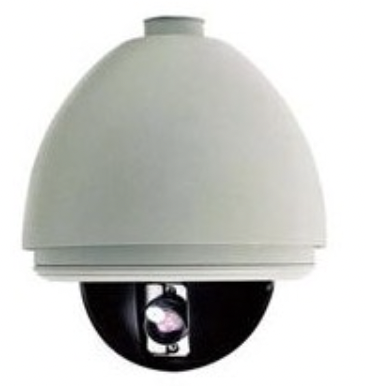
\includegraphics[width=\textwidth / 3]{figsrc/speeddome.png}
    \caption{Speed dome camera\label{fig:speeddome}}
\end{figure}

%     PI
\subsection{Raspberry PI}
Raspberry Pi~\cite{pi} is a series of small single-board computers which is cheaper than standard personal computer as shown in Fig.~\ref{fig:pi}. It is placed in experimental field with Speed dome. PI acts as a edge management device. It recieves command from other servers by MQTT~\cite{mqtt-intro} protocol then commands camera by API request and recording server to execute. Spec of CPU is Quad core, ARM Cortex-A72(v8) 64bytes 1.5GHz and RAM is 4GB LPDDR4-2400 SDRAM and storage is 16 GB MicroSD.

\begin{figure}[H]
    \centering
    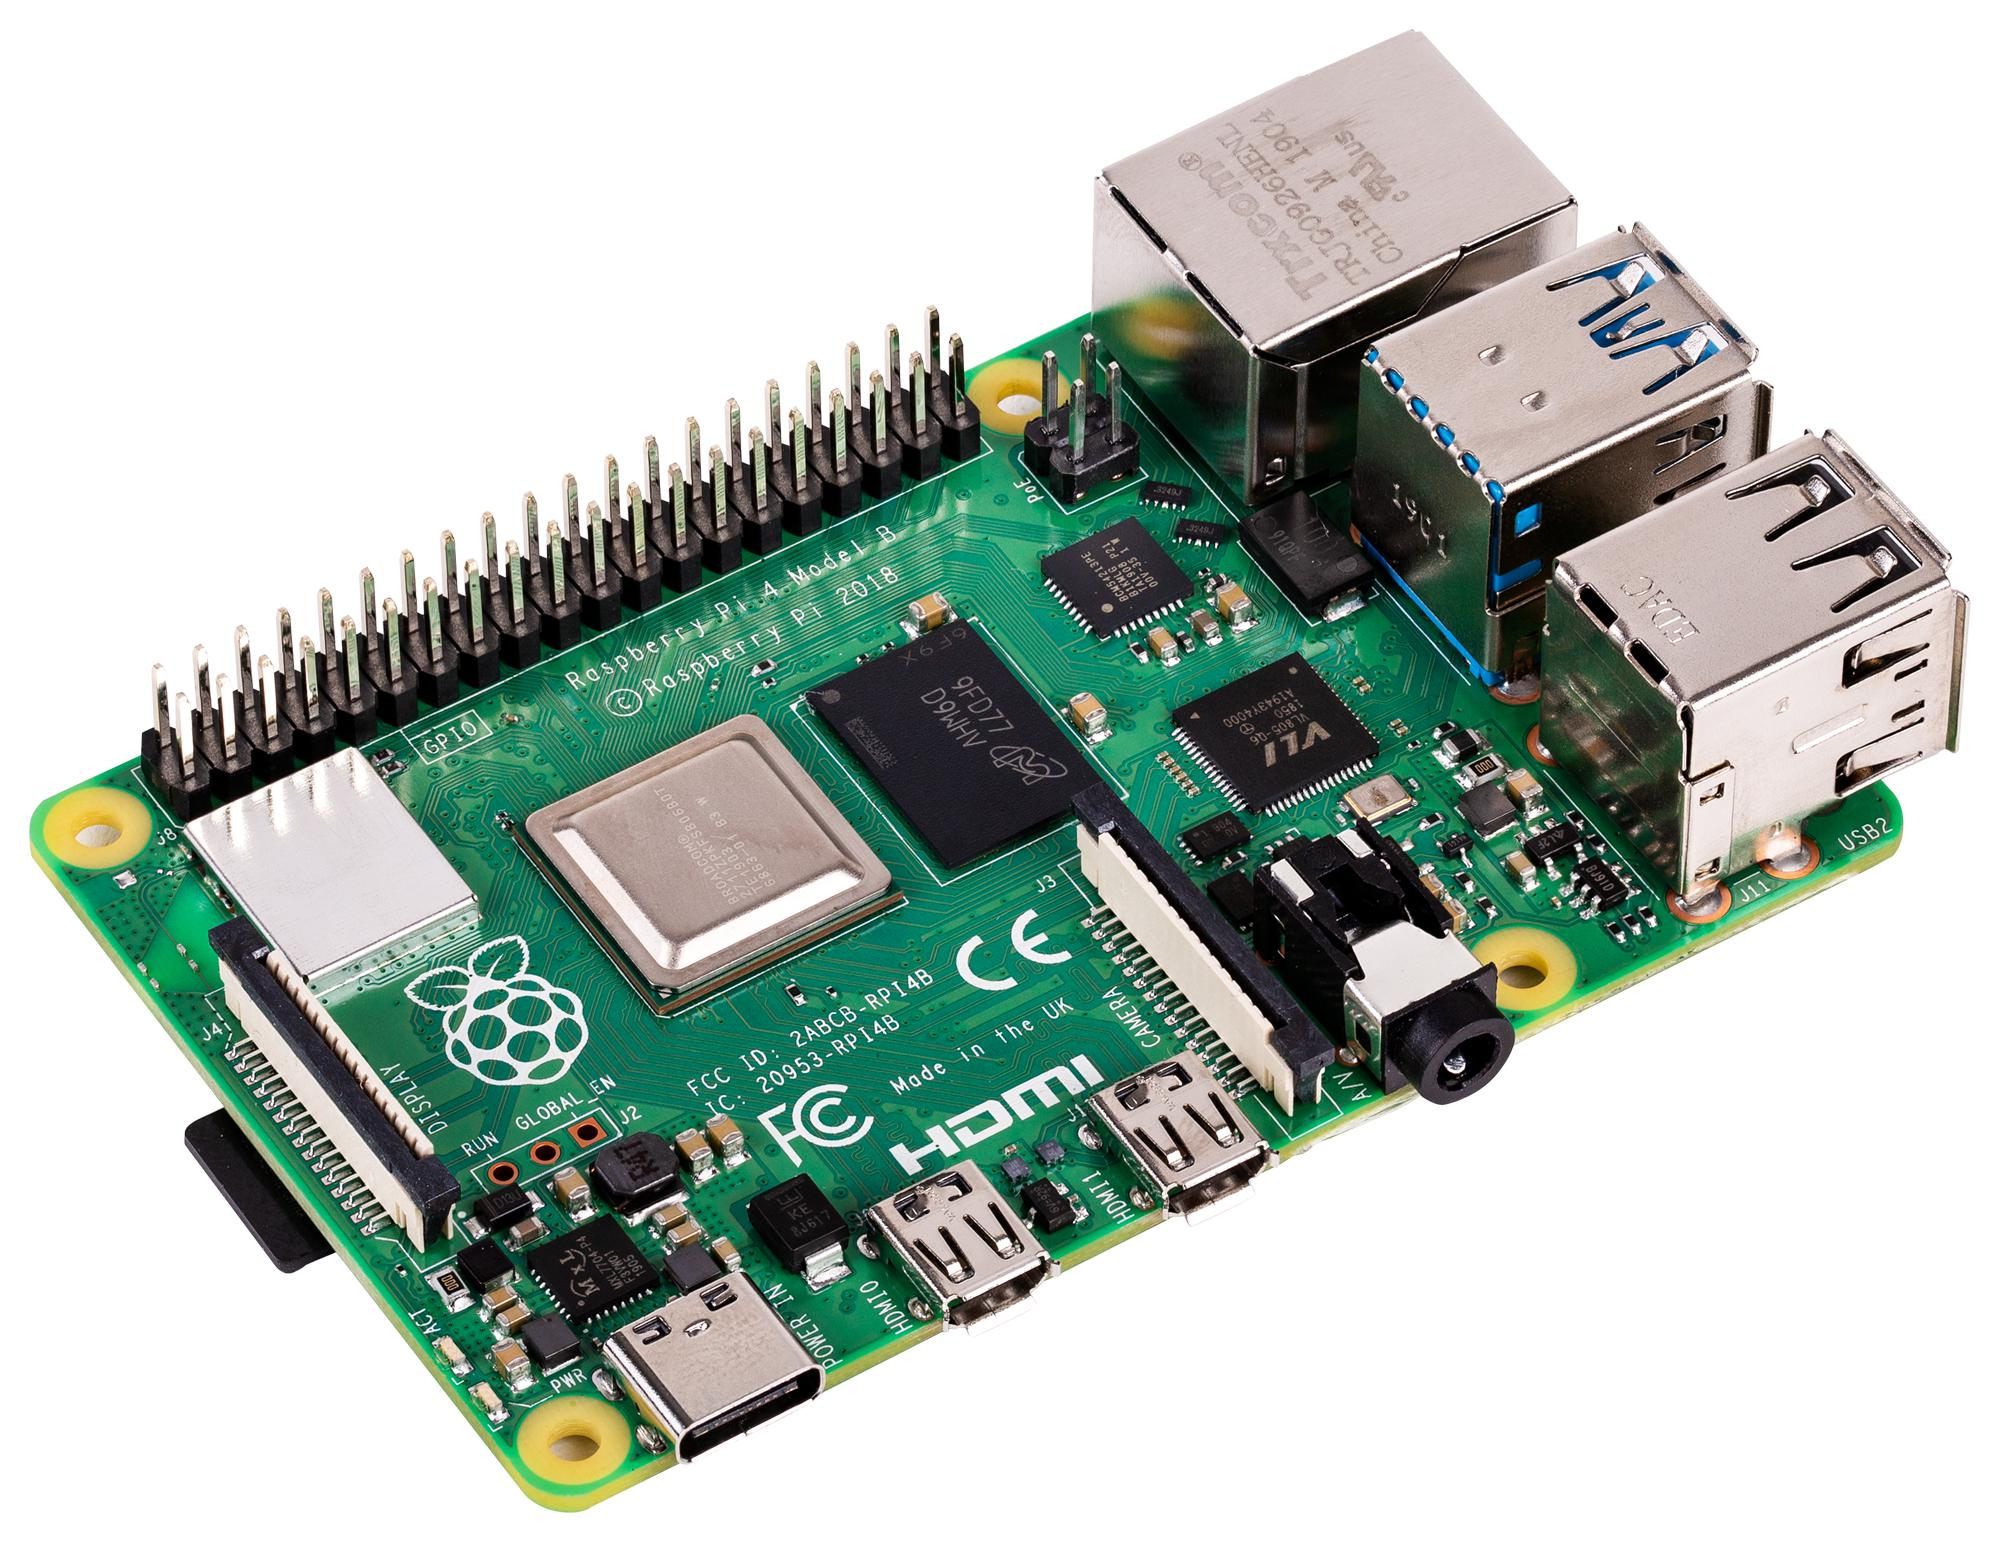
\includegraphics[width=\textwidth]{figsrc/pi.jpeg}
    \caption{Raspberry PI\label{fig:pi}}
\end{figure}

%     % 網路端
%     Video streaming server
\subsection{Video streaming server}
Video streaming server~\cite{ossr} is open sourcing streaming server. It is a simple, high efficiency and realtime video server, supports RTMP/WebRTC/HLS/HTTP-FLV/SRT. It is used to recieve RTMP streaming from Speed dome.

%     recording server
\subsection{Recording server}
Recording server receives command from PI. It is reponsible to pull live streaming from video streaming server then make into video file. After finish recording, it upload file to AWS S3. Our recording process uses the feature of OpenCV~\cite{opencv} as our backbone. It has some advantage such as easy to use, Support multi stream protocol(RTMP, RTSP …etc.) and less bug.

%     API server
%     Front end
%     aws s3
%     aws dynamoDB
\subsection{File Storage and Database}
We utilize AWS S3 to store video file and AWS DynamoDB~\cite{aws-dynamodb} as database. DynamoDB will store various metadata, including scheduled time for record, meta data for PI in edge side.

%     scheduled server
\subsection{Scheduled server}
Scheduled server fetch information from DynamoDB and is responsible to send recording request to PI when some events or specific timing occured. 


%     MQTT broker 
\section{User cases enumeration}
Here, we will show the user cases for our system. We explain how our system work through sequence diagram for each user case.
% 這邊列舉3個user case
% manual
\subsection{Manual case}
In this user case, User will click the recording button in the streaming web page to manually start recording as shown in Fig.~\ref{fig:manual-case}. 


\begin{figure}[H]
    \centering
    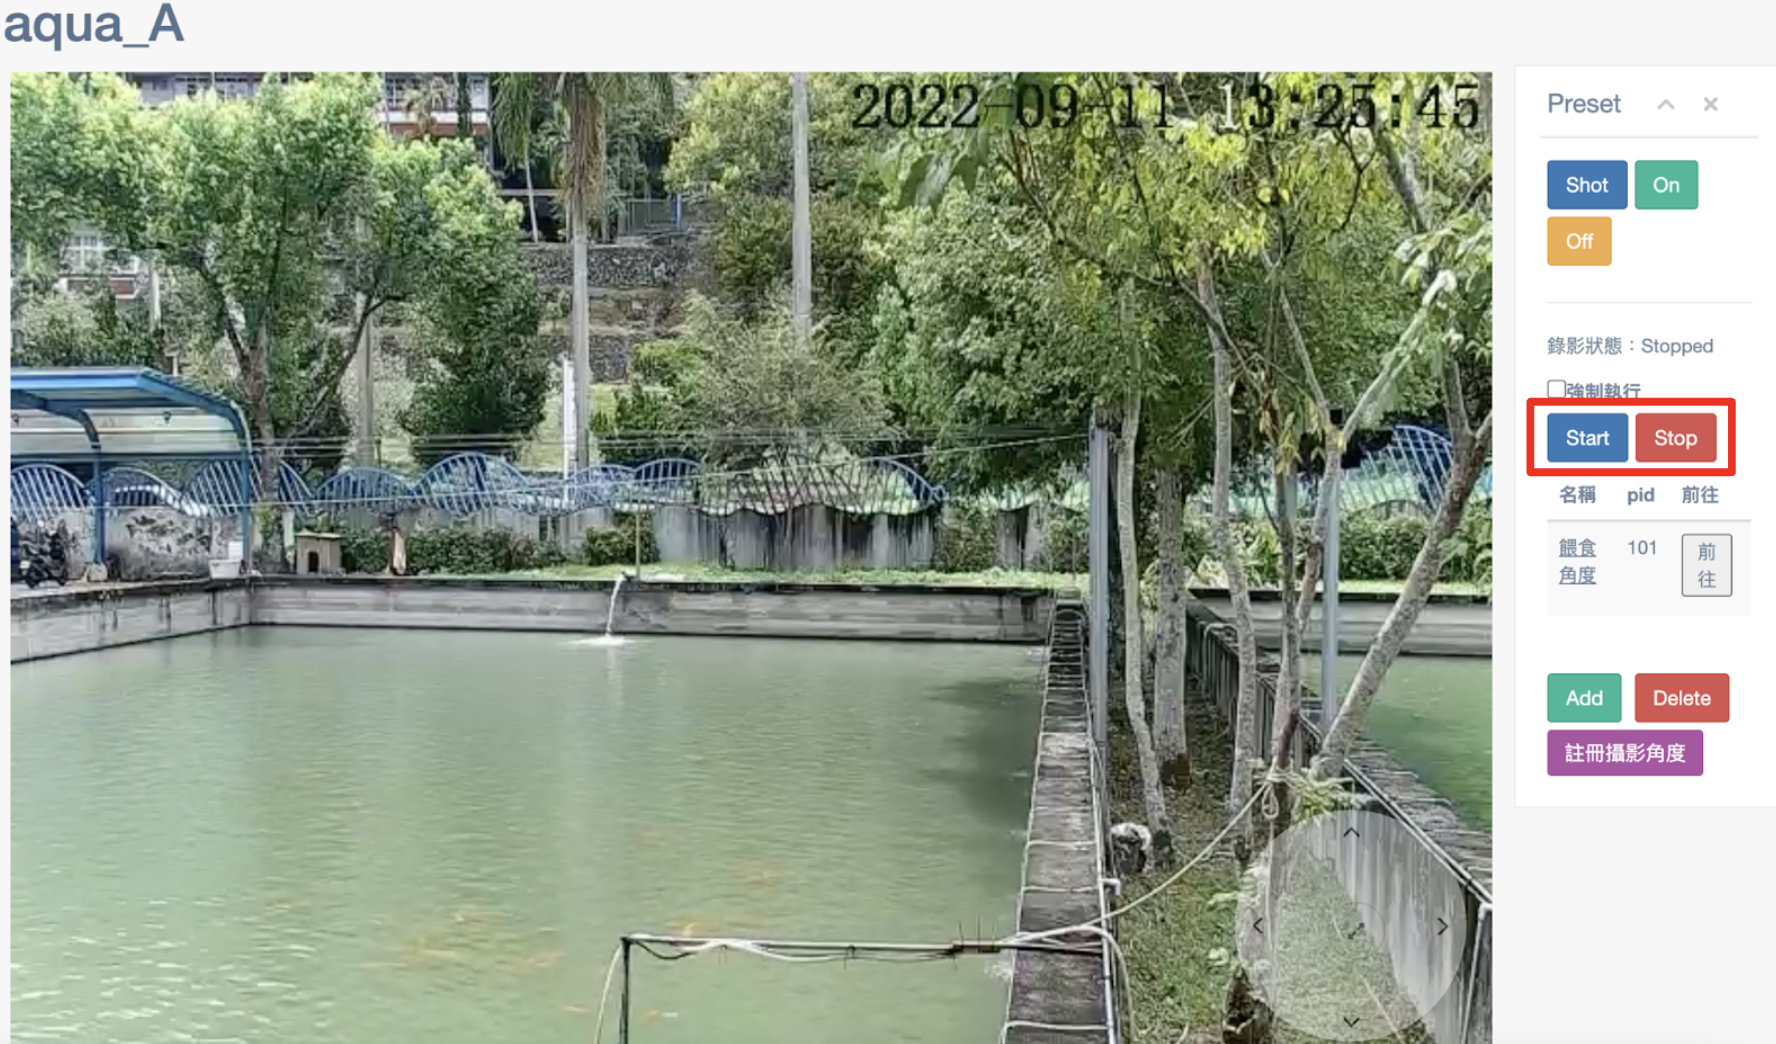
\includegraphics[width=\textwidth]{figsrc/manual-case.png}
    \caption{Click start button to start recording and Press stop button to stop\label{fig:manual-case}}
\end{figure}

As shown in Fig.~\ref{fig:manual-sequece-diagram}, we show the data flow of the whole system from starting the recording task to terminate it. In this manual case, there are 5 components involved, Front-end server, API server(Back-end server), Raspberry PI, Recording system and Video streaming server. When Front-end server sends API request, Back-end will query PI for the permission of the camera. If PI allows the request, it will inform Back-end server that it allows to recieve recording request. Front-end will recieve permission response from Back-end then start to initiate WebSocket~\cite{websocket} connection with Back-end. After WebSocket connection is complete, Back-end will send MQTT record command to PI to start recording process. PI will inform recording server to start connection with streaming server and wait until the connection is complete. Recording system will inform PI that connection is complete then PI will inform recording system to start recording. At the same time, PI will also inform Front-end that the recording process has started. If user want to terminate the recording task, he/she can press the stop button. Front-end will disconnect WebSoceket. When Back-end detect WebSocket connection has been shut down, it will send stop command to inform PI to stop the process. At last, recording system will stop connection with Video streaming server then upload the video file to AWS S3~\cite{aws-s3}.

\begin{figure}[H]
    \centering
    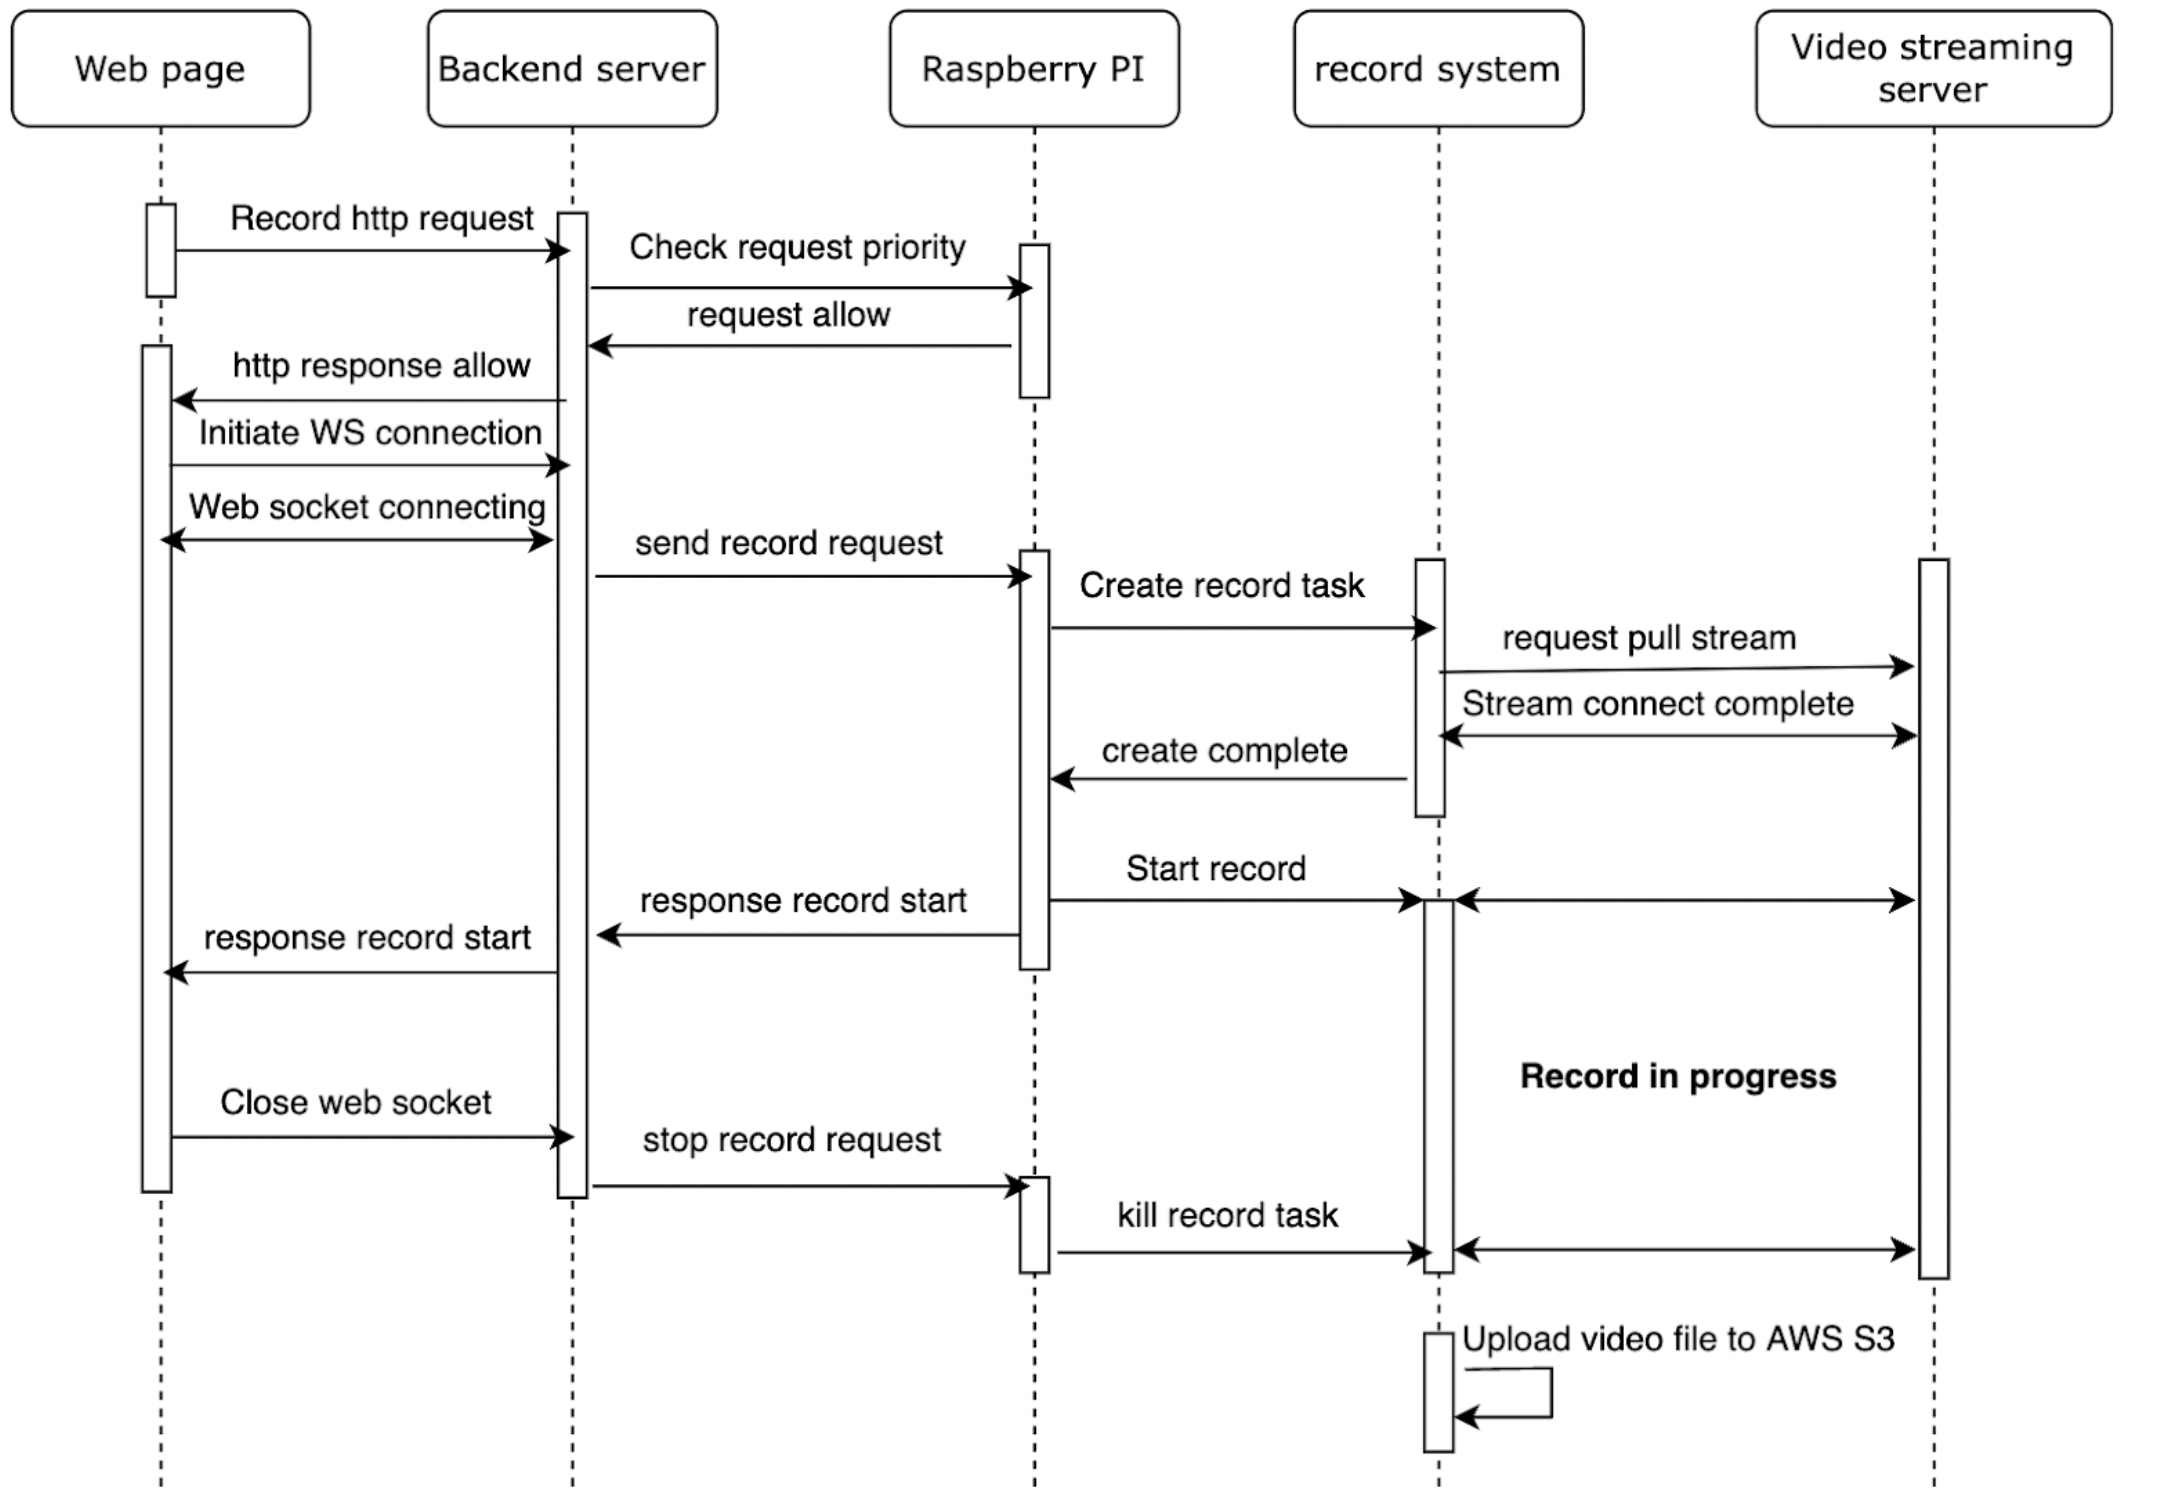
\includegraphics[width=\textwidth]{figsrc/manual-sequece-diagram.png}
    \caption{Data flow of manual case\label{fig:manual-sequece-diagram}}
\end{figure}

% event
\subsection{Event triggered case}
In this case, recording process will start if specific event occured. User have to register the event they want(e.g. Some sensor value exceed specific threshold.) to record. The steps are shown in Fig.~\ref{fig:event-userflow}. First, in Fig.~\ref{fig:event-userflow-a}, user can rotate camera to the angle they want then press the purple button to store the angle. Second, in Fig.~\ref{fig:event-userflow-b}, user can set a name for this angle. Third, in FIg.~\ref{fig:event-userflow-c}, user will set the recording duration, angle name, the type of event.

\begin{figure}[H]
    \centering
    \begin{subfigure}{\textwidth}
        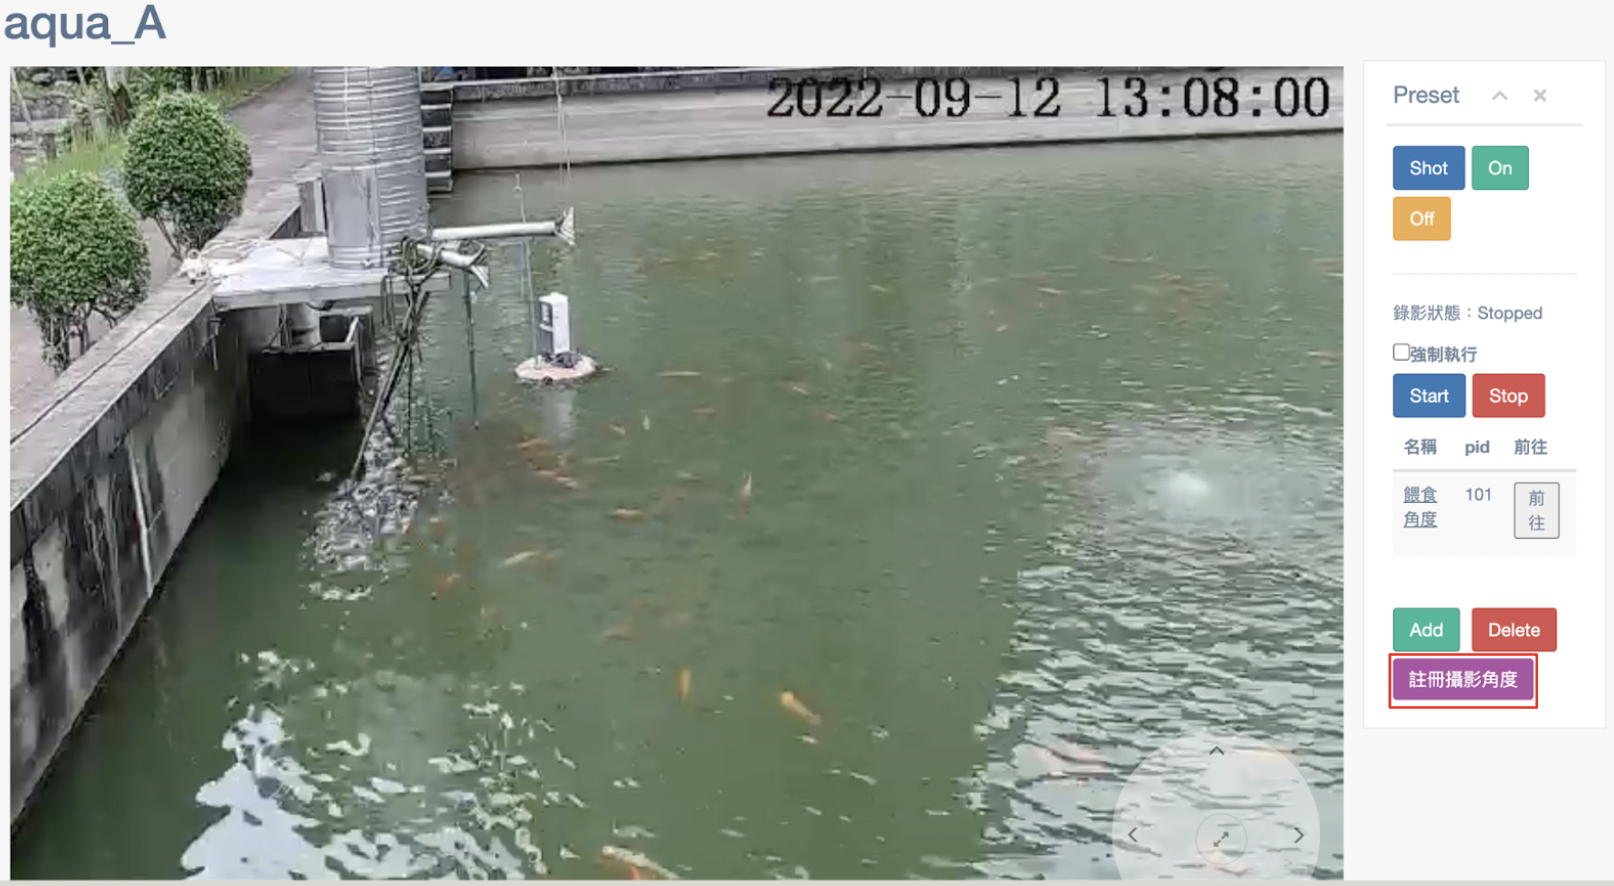
\includegraphics[width=\textwidth]{figsrc/event-userflow-a.png}
        \subcaption{Go to an angle you want}
        \label{fig:event-userflow-a}
    \end{subfigure}

\medskip
    \begin{subfigure}{\textwidth}
        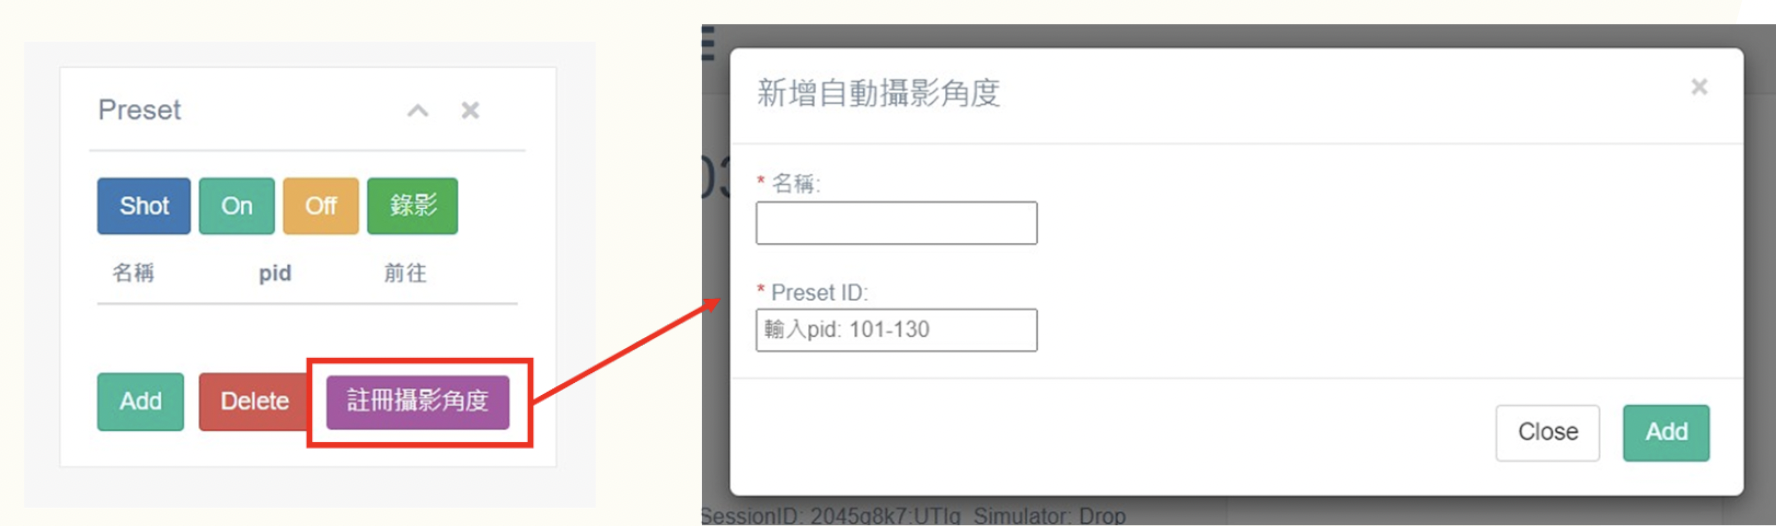
\includegraphics[width=\textwidth]{figsrc/event-userflow-b.png}
        \subcaption{Set a name for this angle}
        \label{fig:event-userflow-b}
    \end{subfigure}
    \caption{User flow of event triggered case}
\end{figure}

\begin{figure}[H]
    \ContinuedFloat
    \centering
    \begin{subfigure}{\textwidth}
        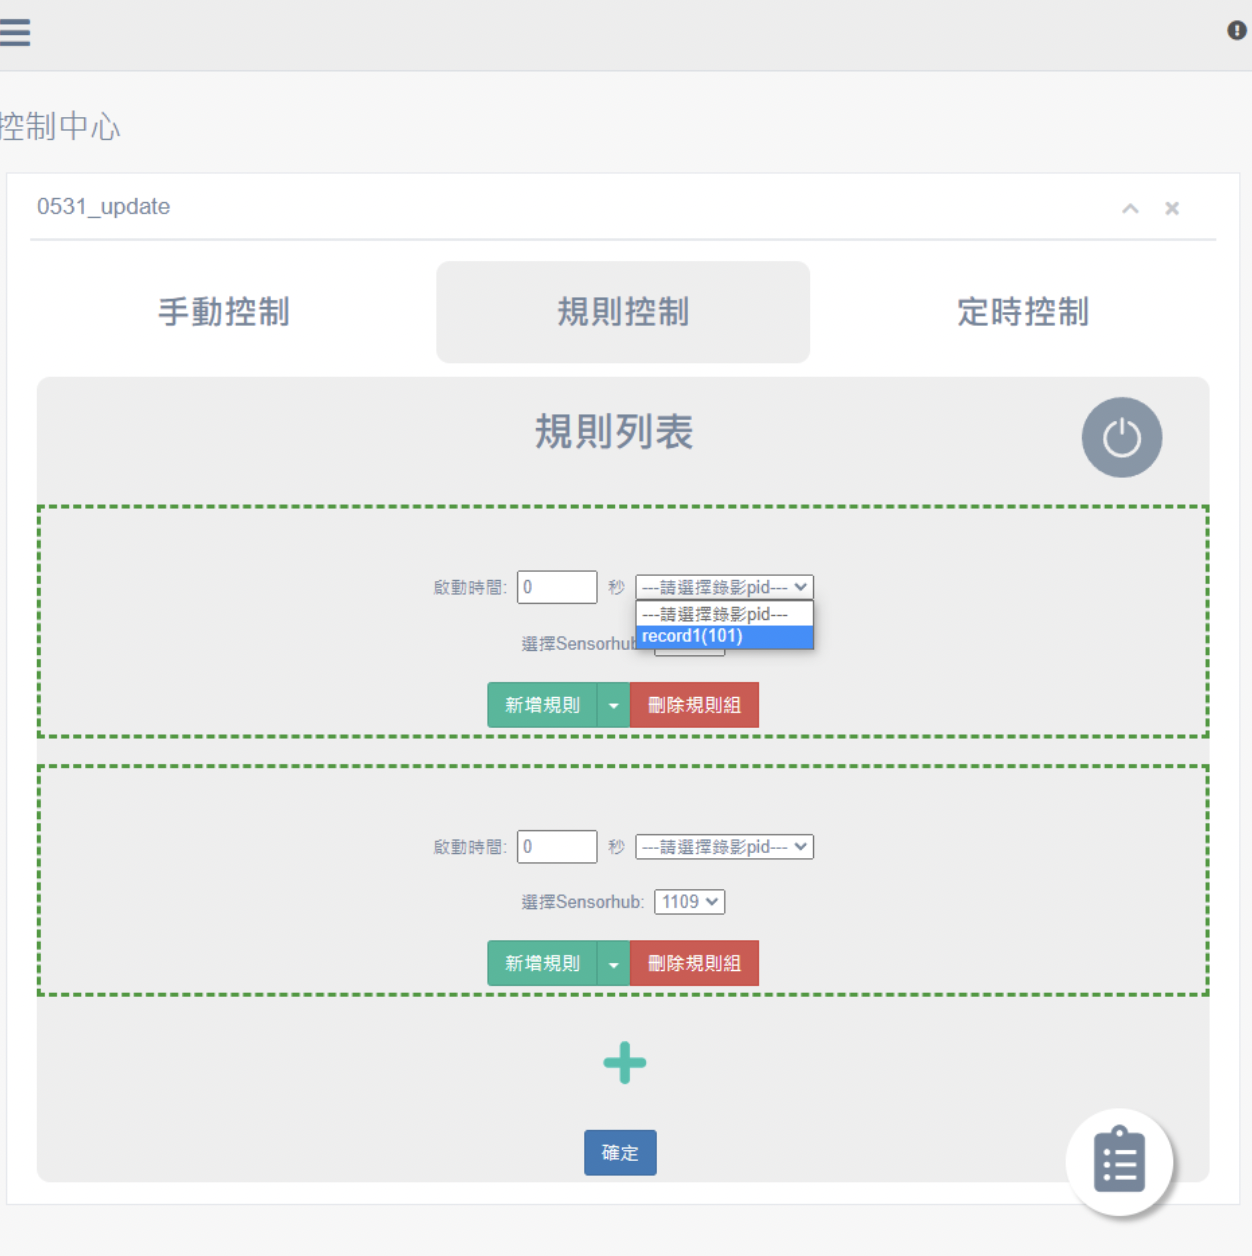
\includegraphics[width=\textwidth]{figsrc/event-userflow-c.png}
        \subcaption{Choose an event}
        \label{fig:event-userflow-c}
    \end{subfigure}

    \caption{User flow of event triggered case(cont.)}
    \label{fig:event-userflow}
\end{figure}

We will also show the sequence diagram of event case below from registering event to recording process terminated in Fig.~\ref{fig:event-sequence-diagram}. In this case, there are 6 components involved, Front-end server, API server(Back-end server), Scheduling server, Raspberry PI, Recording system and Video streaming server. When user register a event, Back-end will send the event information, including camera angle, recording duration and task type, to scheduling server. When event occured, scheduling server will send recording request to recording server. Similar to manual case, PI will inform recording server to start connection with streaming server and wait until the connection is complete. Recording system will inform PI that connection is complete then PI will inform recording system to start recording for X seconds. Recording server will shut down video process when time's up. At last, recording system will stop connection with Video streaming server then upload the video file to AWS S3.

\begin{figure}[H]
    \centering
    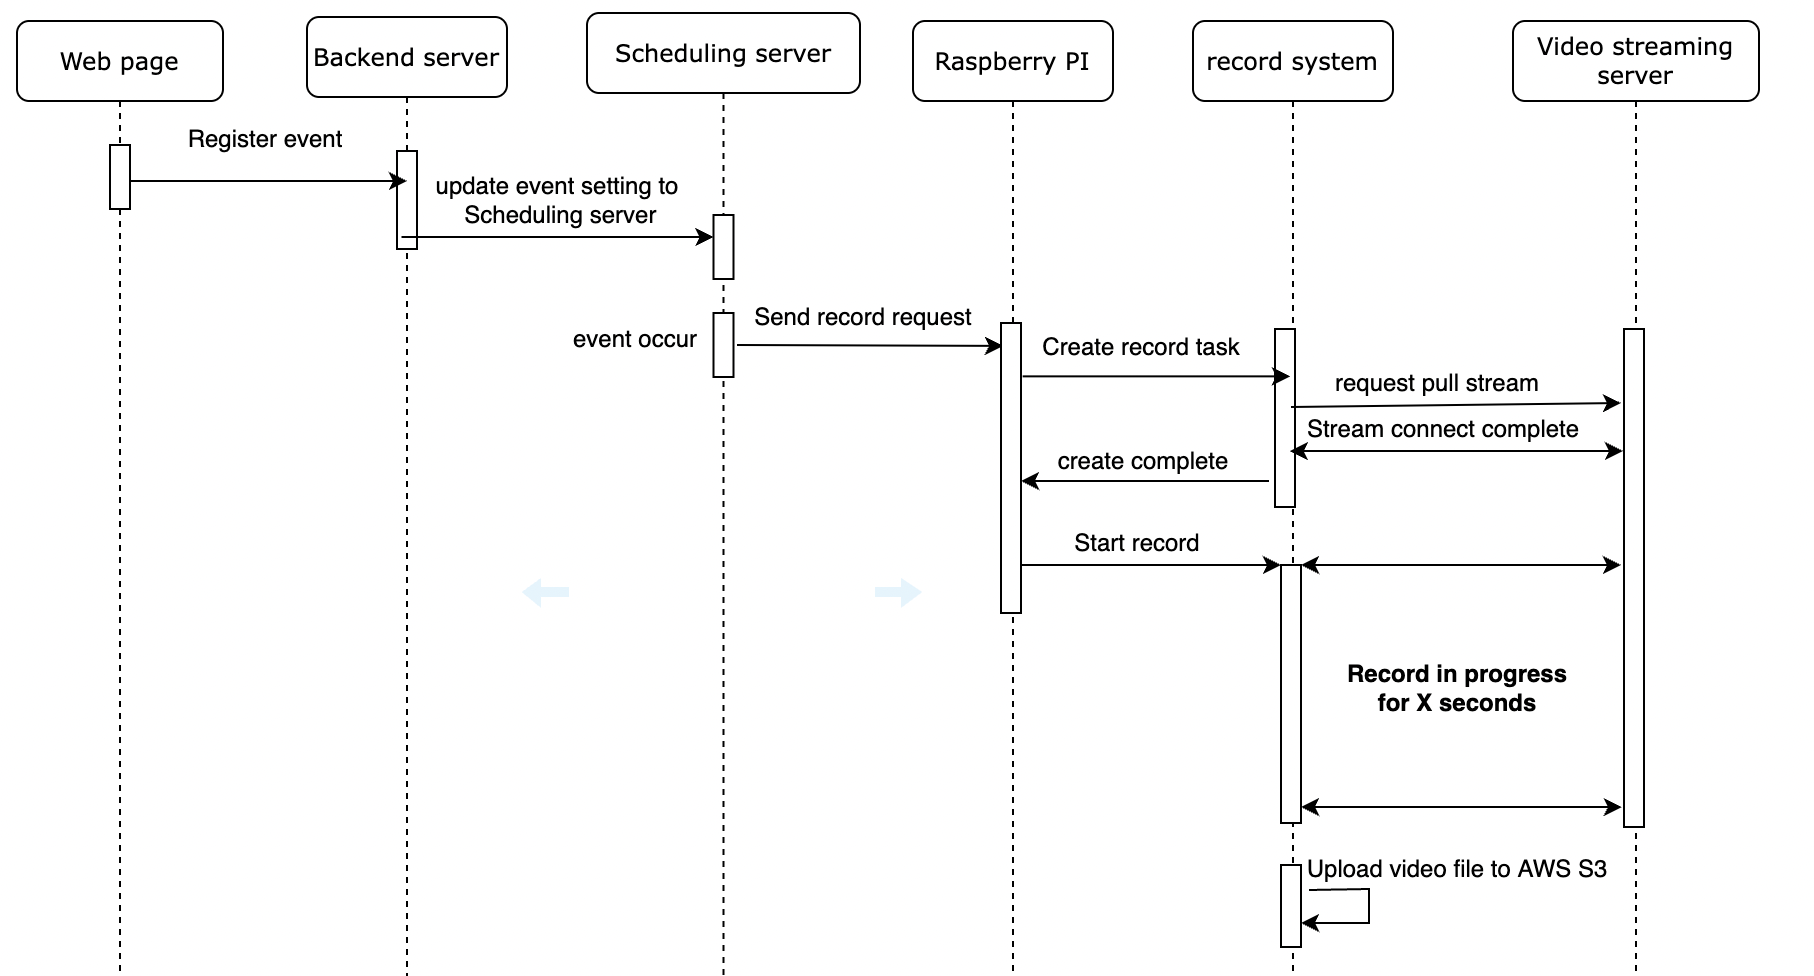
\includegraphics[width=\textwidth]{figsrc/event-sequence-diagram.png}
    \caption{Data flow of event triggered case\label{fig:event-sequence-diagram}}
\end{figure}


% time
\subsection{Time period triggered case}
In this case, record process will be triggered at a specific timing. Similar to event register, as shown in Fig.~\ref{fig:time-userflow-a}, user can rotate camera to the angle they want then press the purple button to store the angle then in Fig.~\ref{fig:time-userflow-b} user can set a name for this angle. At last, in Fig.~\ref{fig:time-userflow-c}, we can set the time period, recording duration and recording angle.

\begin{figure}[H]
    \centering
    \begin{subfigure}{\textwidth}
        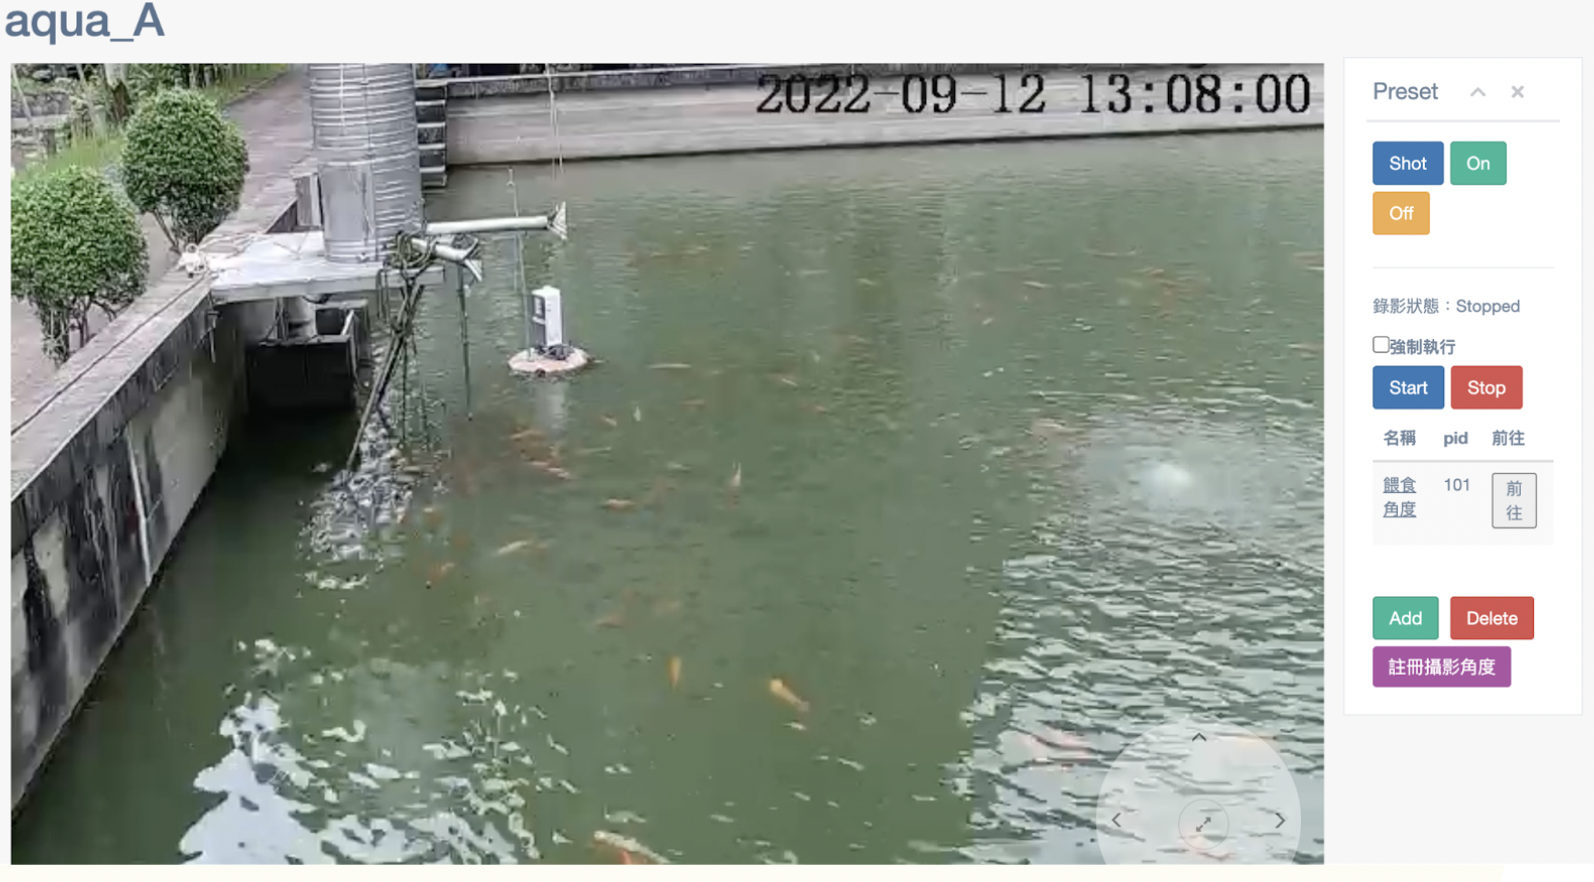
\includegraphics[width=\textwidth]{figsrc/time-userflow-a.png}
        \subcaption{Go to an angle you want}
        \label{fig:time-userflow-a}
    \end{subfigure}

\medskip
    \begin{subfigure}{\textwidth}
        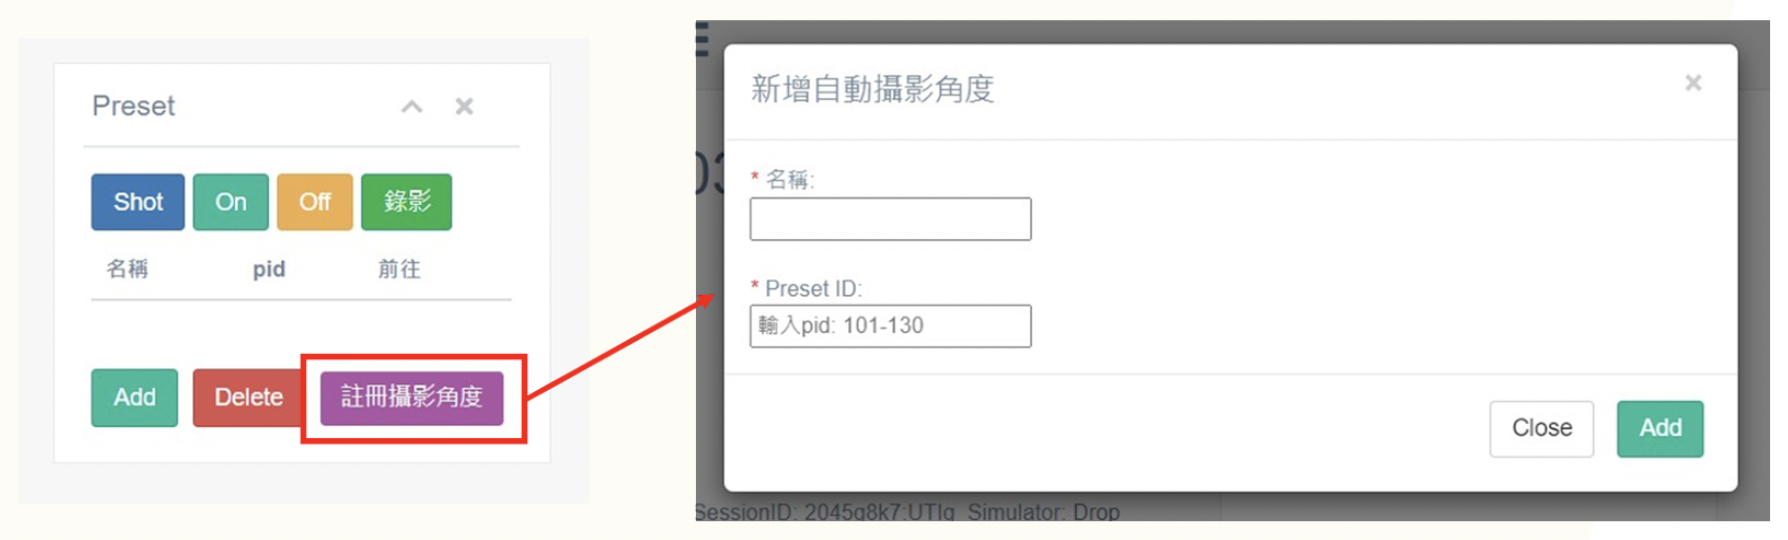
\includegraphics[width=\textwidth]{figsrc/time-userflow-b.png}
        \subcaption{Set a name for this angle}
        \label{fig:time-userflow-b}
    \end{subfigure}
    \caption{User flow of time period triggered case}
\end{figure}

\begin{figure}[H]
    \ContinuedFloat
    \centering
    \begin{subfigure}{\textwidth}
        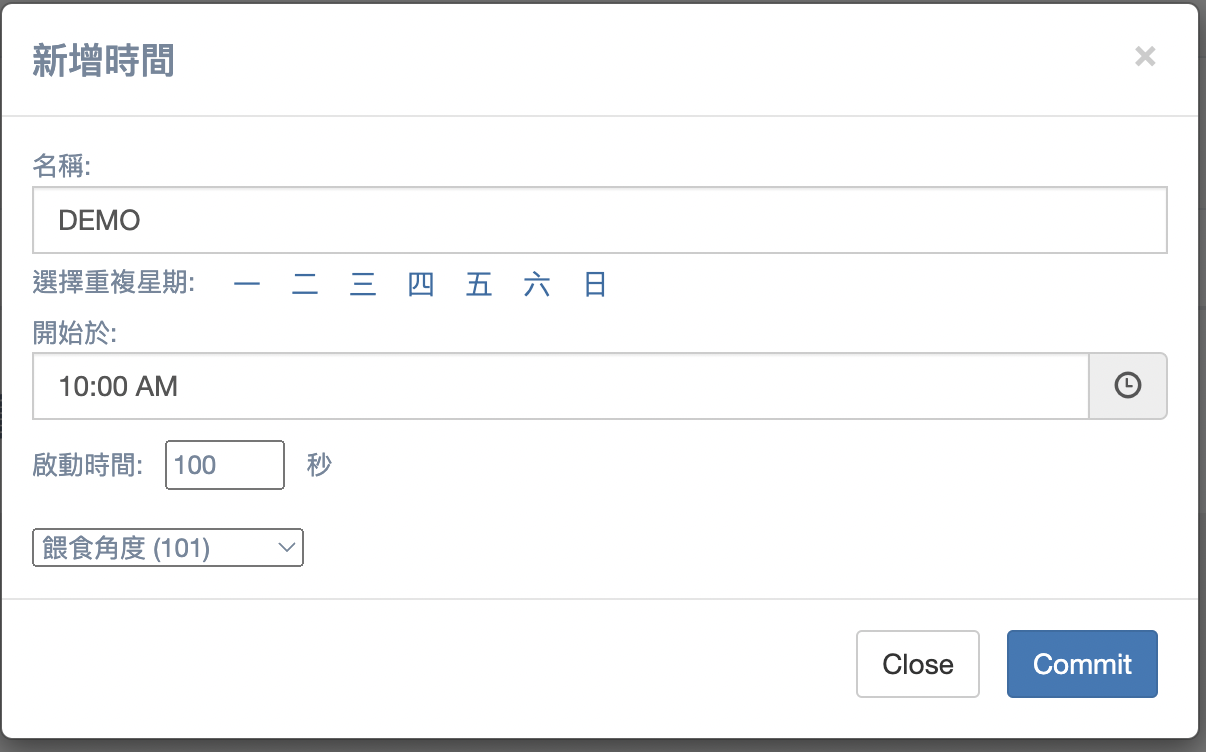
\includegraphics[width=\textwidth]{figsrc/time-userflow-c.png}
        \subcaption{Choose an time}
        \label{fig:time-userflow-c}
    \end{subfigure}

    \caption{User flow of time period triggered case(cont.)}
    \label{fig:time-userflow}
\end{figure}

Similar to event trigger case, it has 6 components, Front-end server, API server(Back-end server), Scheduling server, Raspberry PI, Recording system and Video streaming server. The sequence diagram is shown below. In Fig.~\ref{fig:time-sequence-diagram}, when user reigister time setting, Back-end will update the information whilch is identical to event trigger case except the task ID to schduling server. When the time comes, scheduling server will send recording request to PI then do the exact same process in event triggered case. PI will inform recording server to start connection with streaming server and wait until the connection is complete. Recording system will inform PI that connection is complete then PI will inform recording system to start recording for X seconds. Recording server will shut down video process when time's up. At last, recording system will stop connection with Video streaming server then upload the video file to AWS S3.

\begin{figure}[H]
    \centering
    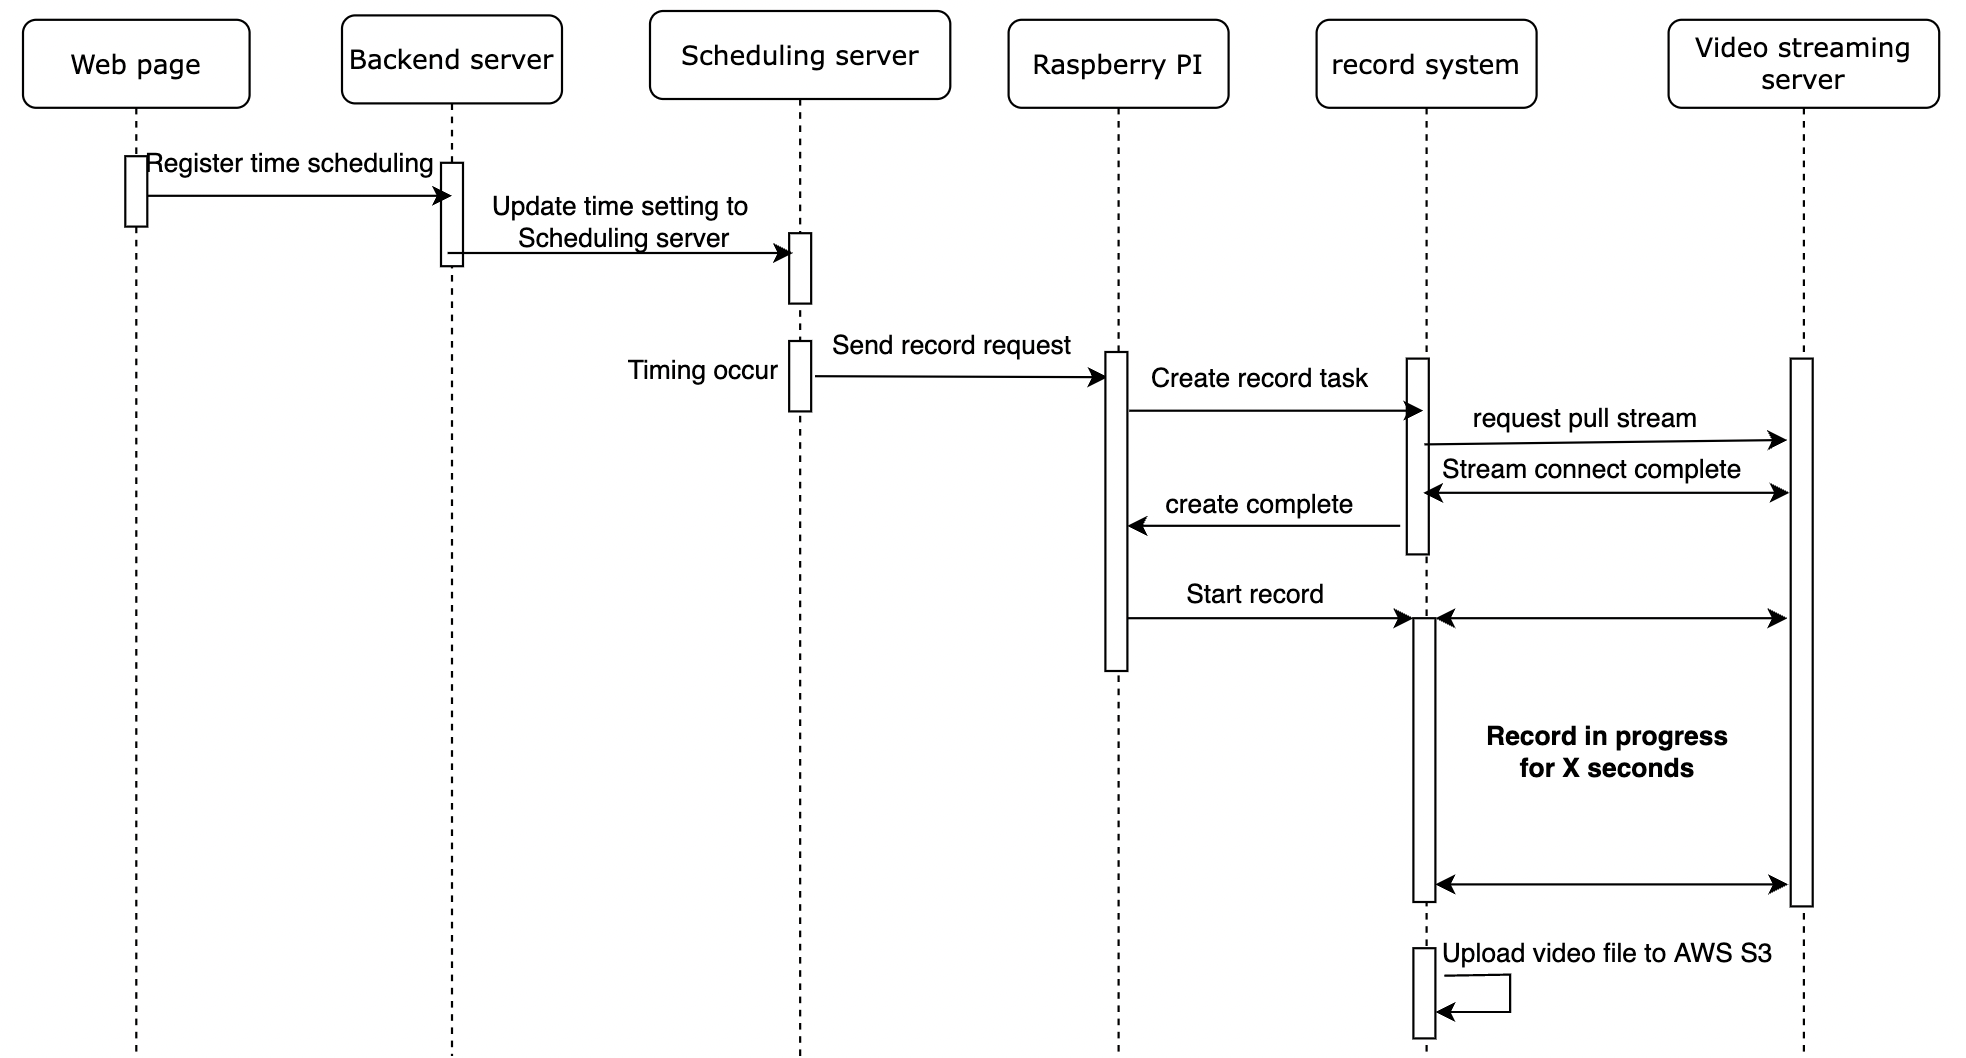
\includegraphics[width=\textwidth]{figsrc/time-sequence-diagram.png}
    \caption{Data flow of time period triggered case\label{fig:time-sequence-diagram}}
\end{figure}

% 1個special case: preemptive
\subsection{Critical case: Preemptive case}
We have shown normal cases that run on our system. Here, we want to point out a special situation. Normally, camera is only capable of executing one recording request. As shown in Fig.~\ref{fig:preemptive-example}, What if there are multiple recording request inbond at the same time?(e.g. At the moment, user A and B want to record manually and an event also trigger the recording process.) It is obvious that camera cannot handle more than one recording request. It doesn't know that which tasks should be executed. We implement priority method to handle such situation in Raspberry PI. If there are multiple cases, PI can check the importance of each task to decide which task can be executed. For example, PI is running task A. Next, task B comes in and request to record. PI will compare the importance, or prioirty, between task A and B. If B is lower than A, PI will reject the request from B. If B is higher than A, PI will stop task A and turn the permission to task B.


\begin{figure}[H]
    \centering
    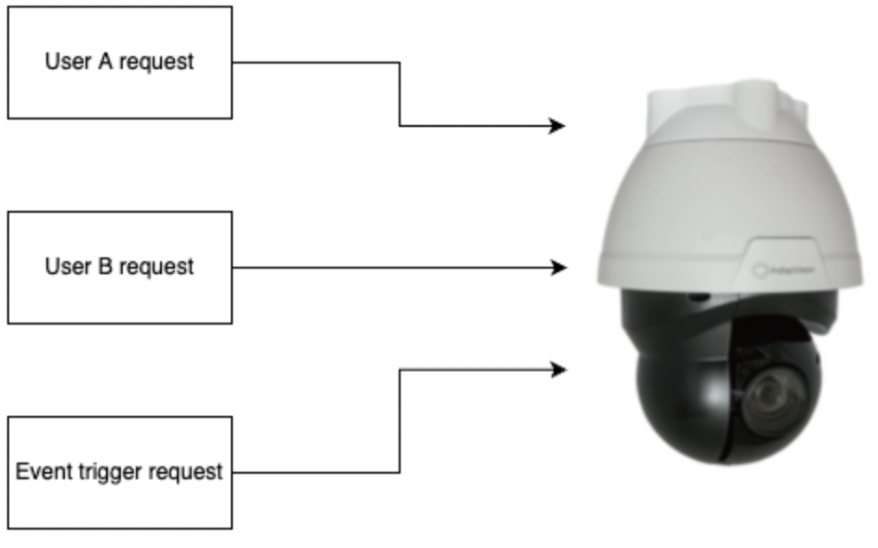
\includegraphics[width=\textwidth]{figsrc/preemptive-example.png}
    \caption{3 requests come at the same time \label{fig:preemptive-example}}
\end{figure}

% PI
% record system


